\textit{Cette phase d'analyse est un élément indispensable à la bonne réalisation du projet. Dans un premier temps, un modèle plus fidèle à la réalité des schémas stockés dans les SGBDR est présenté. Cette partie est suivie d'une petite réflexion sur l'utilisation des ORM. Sont ensuite parcourues les solutions de génération de graphes pour la représentation des données. Les choix concernant l'interface utilisateur seront également exposés.}

\section{Le modèle}
\subsection{Modèle réellement rencontré}

Lors de l'étude des métadonnées stockées par les différents SGBD, nous avons remarqué quelques divergences par rapport au modèle fourni avec le sujet (figure~\ref{figure:diag_classe_fournit} page~\pageref{figure:diag_classe_fournit}). La figure~\ref{figure:diag_classe_reel} présente le diagramme de classes construit suite à nos recherches.

\begin{figure}[H]
\centering
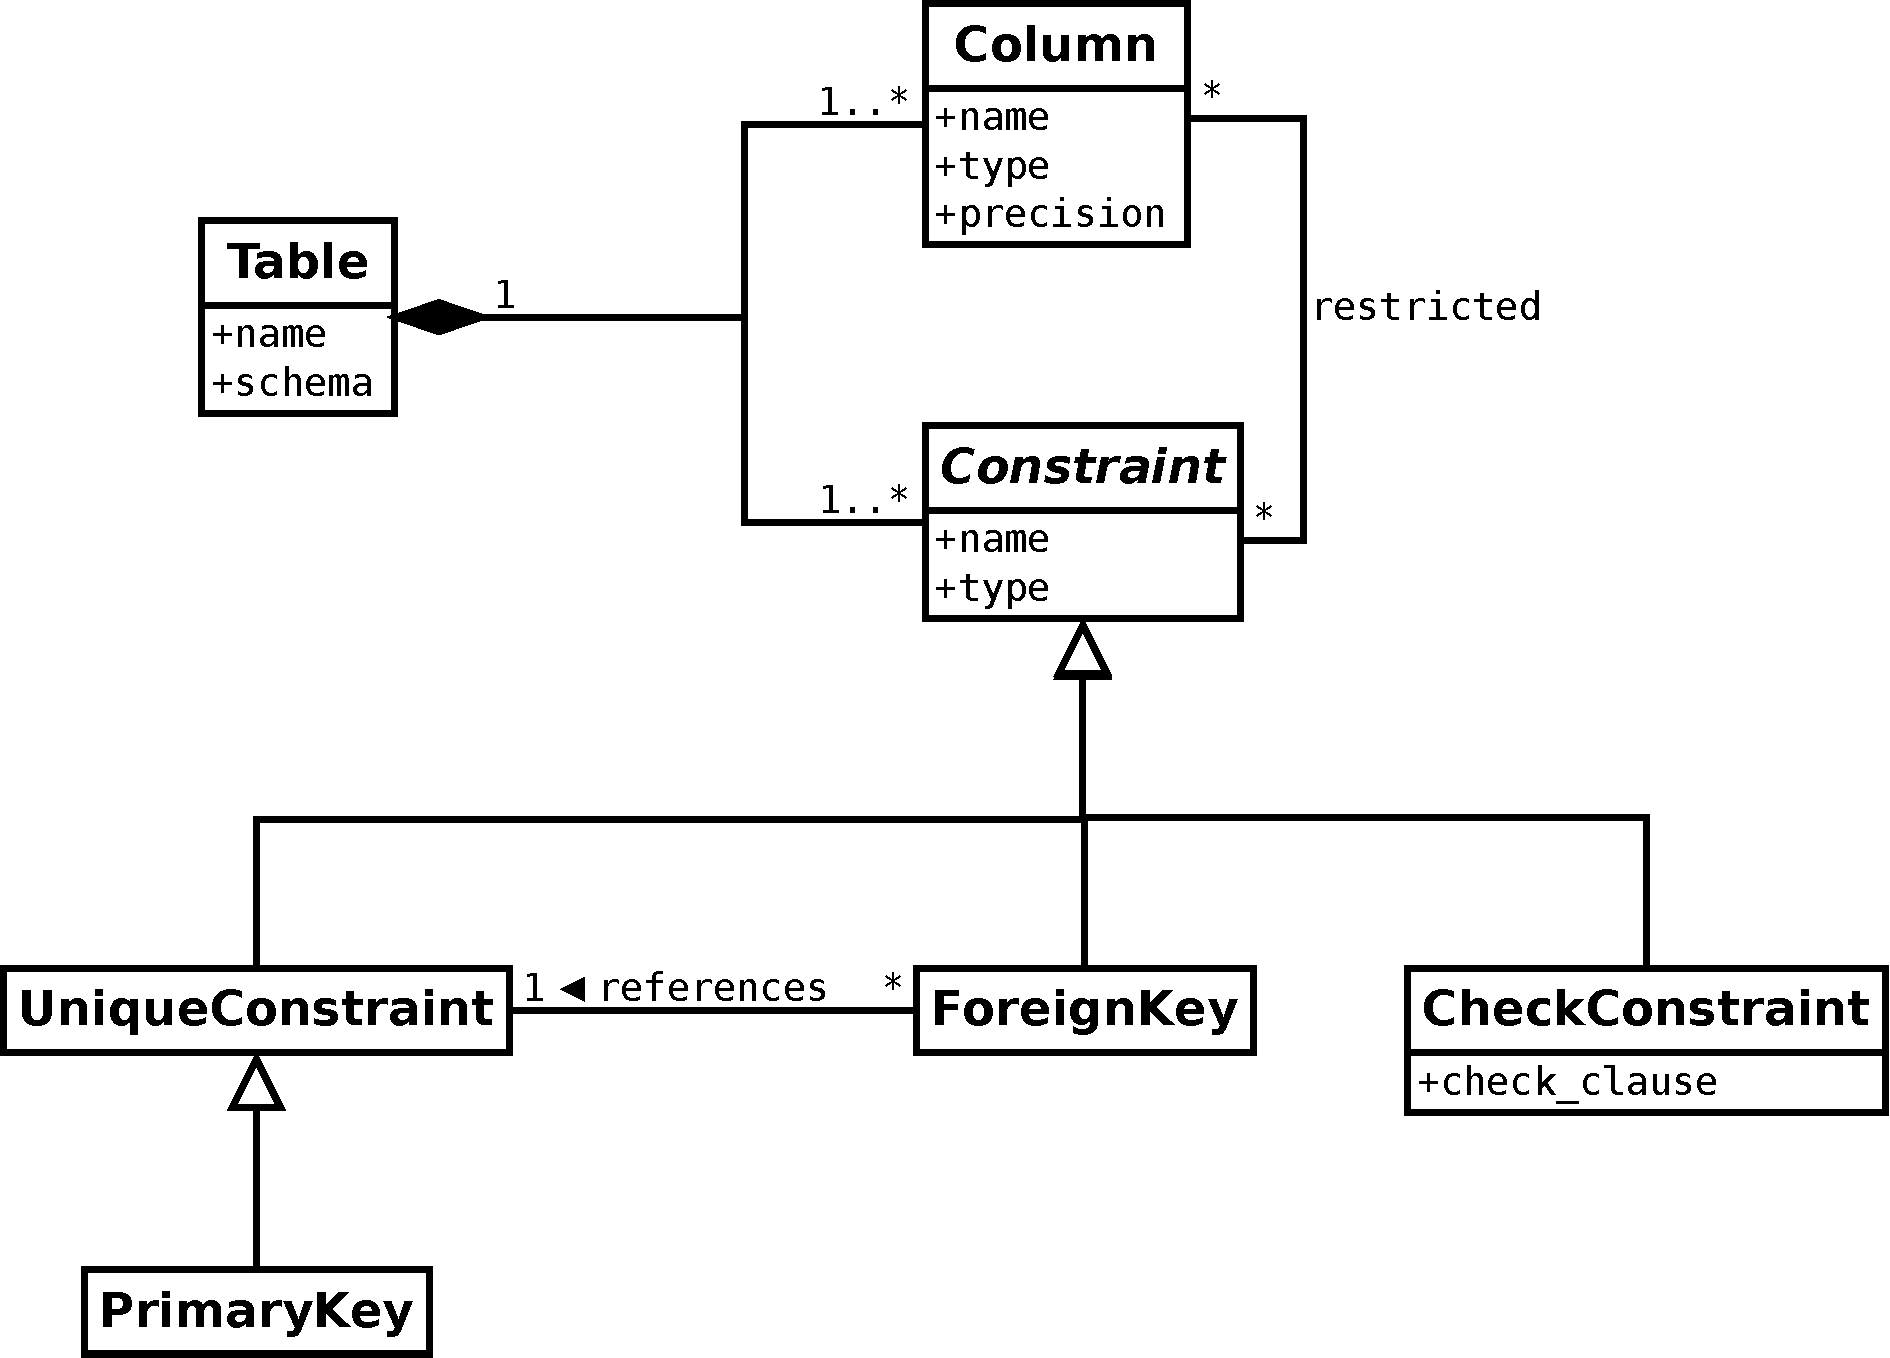
\includegraphics[width=\textwidth]{files/diag_class_ameliore}
\caption{Diagramme de classe réellement rencontré.}
\label{figure:diag_classe_reel}
\end{figure}

La principale différence réside dans la classification des contraintes. Cette classification permet de distinguer trois types de contraintes :

\begin{itemize}
\item Les contraintes d'unicité : elles contraignent l'unicité d'un ou plusieurs attributs au sein d'une même table. Les contraintes de clé primaire sont des contraintes d'unicité.
\item Les contraintes d'intégrité référentielle : elles identifient un ou plusieurs attributs d'une table comme référençant un ou plusieurs attributs d'une autre table, au travers d'une contrainte d'unicité. Notons que ce type de contrainte permet de \textbf{référencer une contrainte d'unicité et non plus une contrainte de clé primaire} comme proposé dans le modèle original.
\item Les contraintes de vérification : qui s'appliquent à un ou plusieurs attributs d'une table. Elles contiennent une clause de vérification \texttt{check\_clause}.
\end{itemize}

\paragraph*{NB}
Les autres types de contraintes (\emph{NULL}, \emph{NOT NULL}, \emph{DEFAULT}, etc.) sont ignorées.

	\subsection{Tables}
		Une table est identifiée par son nom et le schéma auquel elle appartient. Elle possède un ensemble de colonnes et un ensemble de contraintes.
	\subsection{Colonnes}
		Une colonne est identifiée par son nom et la table à laquelle elle appartient. Elle possède un type, et éventuellement une précision. 
	\subsection{Contraintes}
		Une contrainte est identifiée par un nom, sur certains SGBDR il faut lui adjoindre le nom de la table sur laquelle elle est appliquée pour avoir une identification unique (notamment MySQL). Une contrainte possède un type et s'applique sur une ou plusieurs colonnes d'une table. Elle peut être de type clé primaire, clé étrangère, contrainte d'unicité ou contrainte de vérification. Les contraintes d'intégrité référentielles référencent une contrainte de type unique compatible, c'est à dire que les colonnes sur lesquelles s'applique la clé étrangère et les colonnes sur lesquelles s'applique la contrainte référencée sont au même nombre et de mêmes types.
		
\section{ORM}

	\subsection{Qu'est-ce qu'un ORM?}
    Un ORM ou \emph{mapping objet-relationnel} (en anglais \emph{object-relational mapping}) est une méthode de programmation qui consiste à donner l'illusion d'une base de données orientée objet à partir d'une base de données relationnelle en implémentant une interface entre celle-ci et le code de l'application. Il permet donc de palier aux problèmes d'adaptation entre le paradigme objet et les SGBDR en remplaçant les accès à la base de données par des appels à des méthodes objet de haut niveau.
   
	\subsection{Pourquoi?}
    Les systèmes de gestion de bases de données orientées objet étant actuellement peu nombreux et la norme SQL3 n'étant que partiellement implémentée, les ORM offrent à ce jour le meilleur compromis entre la performance des SGBDR et le pouvoir expressif de la modélisation objet.
    
En revanche, cette méthode d'abstraction présente l'inconvénient de générer un schéma différent de la vision objet avec laquelle est modélisée l'application. Il peut parfois être nécessaire d'intervenir directement sur la base de données (développement de TRIGGERS, dump SQL, \ldots), ce qui nécessite alors un effort d'analyse et de compréhension.

\section{Compatibilité avec les SGBDR}
	\subsection{Fichiers de configuration}
	Dans un but d'extensibilité, chaque type de SGBDR possédera un répertoire contenant ses propres fichiers de configurations. Pour chacun, un premier fichier permettra de définir les principaux paramètres pour se connecter et dialoguer avec celui-ci, un second définira les paramètres pour le mapping effectué par \emph{Hibernate} entre le modèle objet et l'organisation des méta-données du SGBDR.

	\subsection{Gestion des types génériques}
	\label{section:generic_types}
	L'application se trouve confrontée à deux sortes de types : les types de données (attributs), et les types de contraintes. Bien qu'étant globalement normés, certains types de données fournis par les SGBDR n'appartiennent pas à la norme \texttt{SQL} . Nous avons donc choisi de mettre en place une stratégie de déclaration de types génériques. Pour chaque SGBDR compatible, chaque type générique est associé à un ou plusieurs types réels du SGBDR.
	
	Cela permet, pour un même schéma relationnel, d'obtenir le même résultat quel que soit le SGBD à partir duquel est chargé le schéma.

\section{Visualisation de graphes}
	
	Nous souhaitons avoir une représentation la plus proche possible d'une représentation connue de schéma de base de données afin que celle-ci soit rapidement compréhensible par des personnes averties. Pour ce faire nous avons à notre disposition plusieures librairies permettant l'organisation et la visualisation de graphes.

  \subsection{Librairies possibles}
  	\subsubsection{Graphviz} \textit{Graph Visualization Software}
  	
			GraphViz est un logiciel de visualisation de graphes écrit en C. C'est un logiciel libre sous EPL\footnote{EPL, Eclipse Public Licence.} développé par AT\&T et les laboratoires Bell. Il offre différents algorithmes de spatialisation. Il est à l'origine du langage de description de graphe DOT. C'est un des logiciels les plus utilisés pour l'affichage de graphes, il permet notamment l'affichage de nœuds représentés sous une forme complexe. De plus, il offre une interface en ligne de commande\footnote{voir \texttt{man graphviz}} aisément utilisable par un programme tiers.
		\subsubsection{JUNG} \textit{Java Universal Network/Graph Framework}
		
				JUNG est une API java permettant la modélisation, l'analyse et la visualisation de graphes. C'est un logiciel libre sous licence BSD\footnote{voir http://jung.sourceforge.net/license.txt} qui est développé par l'université de Californie. Cette API semble bien fournie et documentée, mais ne semble pas être en mesure d'afficher des nœuds aux formes complexes. 
		\subsubsection{Grappa} \textit{A Java \texttt{gra}ph \texttt{pa}ckage}
		
			Grappa est une API java de visualisation et manipulation de graphes. C'est un logiciel libre sous CPL\footnote{CPL, Common Public Licence.} développé par John Mocenigo d'AT\&T. Cette API se base sur le langage de description de graphe DOT et est partiellement compatible pour l'affichage des nœuds de formes complexes.
		
				
  \subsection{Notre choix}
		Notre choix s'est porté sur GraphViz, et plus particulièrement sur la commande \texttt{dot} qui offre un algorithme de spatialisation hiérarchique. GraphViz présente les principaux avantages d'être extrêmement simple d'utilisation grâce à son interface en ligne de commande et d'offrir la possibilité de générer des nœuds de formes complexes ce qui nous permettra de nous rapprocher d'une représentation d'une entité du formalisme E/A\footnote{Entité/Association}.

\section{L'IHM}	
	\subsection{Les choix possibles}
	\label{ihm_choix_possibles}
		Notre Interface Homme-Machine peut être conçue de deux manières. La première solution consiste en la création d'une interface graphique proposant une fenêtre de configuration puis un affichage du résultat obtenu. La seconde est orientée ligne de commande générant une image représentant le résultat. 	
	
		\subsubsection{GUI : \og Graphical User Interface \fg{}}
			Une interface utilisateur graphique permet une prise en main rapide et intuitive d'un logiciel mais ne permet pas une grande interopérabilité. En effet, il est compliqué de demander à un programme de configurer un autre programme via une interface graphique.
			
		\subsubsection{CLI : \og Command Line Interface \fg{}}
			La conception d'une interface en ligne de commande entre dans la philosophie KISS, \og Keep it simple, Stupid! \fg{}. Cette philosophie préconise la recherche de simplicité dans la conception et insiste sur le fait que toute complexité non nécessaire devrait être évitée. Le choix d'une interface en ligne de commande permet de se concentrer sur le cœur de l'application, aussi appelé \og processus métier \fg{}. Cette vision a aussi l'avantage d'offrir une grande interopérabilité, il est en effet aisé d'exécuter une ligne de commande depuis un logiciel tiers et d'en récupérer la sortie. Par contre, une interface en ligne de commande est plus difficile à prendre en main pour un utilisateur non averti.  
			
	\subsection{Notre choix}
		Nous avons choisi pour notre application d'implémenter une interface en ligne de commande pour les avantages détaillés précédemment dans la section~\ref{ihm_choix_possibles}, à savoir sa simplicité et sa grande interopérabilité. De plus, si le besoin d'une interface graphique se fait sentir, pour toucher un public moins averti par exemple, il est toujours possible, à partir de l'interface en ligne de commande, de créer une interface graphique dans un langage quelconque qui encapsulera notre logiciel, alors que l'inverse serait bien entendu beaucoup moins évident.

